\documentclass{article}

\usepackage{scribe}

\setseriestitle{Probabilistic Machine Learning}
\setscribecode{1}
\setauthname{Gurpreet Singh}
\setinstrname{Piyush Rai}
\setheaddate{October 18, 2017}
\settitle{Approximate Inference and Sampling Methods}

\begin{document}
\makeheader%

\begin{ssection}{Locally Conjugate Models}

	Inference with multiple unknows (parameters or hyperparameters) becomes tricky, and usually have intractable posteriors as well. Special methods such as EM or MLE-II have to be used. \br%

	We can approximate these posteriors using the ideo of \textbf{local} or \textbf{conditional conjugacy}. Essentially, the routine is to update one parameter keeping others fixed (similar to EM).

	\begin{ssubsection}{Local Conjugacy}

		Often is the case that the overall posterior $\prob{\vTheta \pipe \vX} = \frac{\prob{\vx \pipe \vTheta} \prob{\vTheta}}{\prob{\vX}}$ is intractable. We define the conditional probability of a parameter $\Theta_k$ as follows

		\begin{align*}
			\prob{\Theta_k \pipe \vX_k, \vTheta_{-k}} = \frac{\prob{\vX_k \pipe \Theta_k, \vTheta_{-k}} \prob{\Theta_k}}{\int \prob{\vX_k \pipe \Theta_k, \vTheta_{-k}} \prob{\Theta_k} d\Theta_k}
		\end{align*} \br%

		\note{Here, $\vTheta_k$ is the set of all parameters excluding $\Theta_k$ and $\vX_k$ is the data that is dependent on $\Theta_k$} \br%

		Suppose the conditional posteriors (CP) admit \textbf{local conjugacy} \textit{i.e.} the above term is tractable for all parameters. Such models are called locally conjugate models.

	\end{ssubsection}

	\begin{ssubsection}{Bayesian Matrix Factorization}

		We assume the data to be modelled as a low rank matrix with some noise term. We need to factorize this $N \times M$ matrix ($\vR$) into two matrices (interpreted as users and items) $\vU$ and $\vV$ of sizes $N \times K$ and $K \times M$ respectively such that $K \ll N, M$ and $\vR \approx \vU \times \vV$ \br%

		We assume the error term, and hence the likelihood to be gaussian

		\begin{align*}
			\vR				&\eq \vU \vV + \vepsilon \\
			r_{ij}			&\eq \vu_i^T \vv_j + \eps_{ij}
			\prob{r_{ij}}	&\eq {r_{ij} \pipe \vu_i^T \vv_j , \beta^{-1}}
		\end{align*} \br

		We assume Gaussian priors on the user and item latent features

		\begin{align*}
			\prob{\vu_i}	&\eq \ND{\vu_i \pipe \vzero, \lambda_u^{-1} \vI_{K}} \\
			\prob{\vv_j}	&\eq \ND{\vv_j \pipe \vzero, \lambda_v^{-1} \vI_{K}}
		\end{align*} \br%

		\begin{figure}[h!]
			\centering
			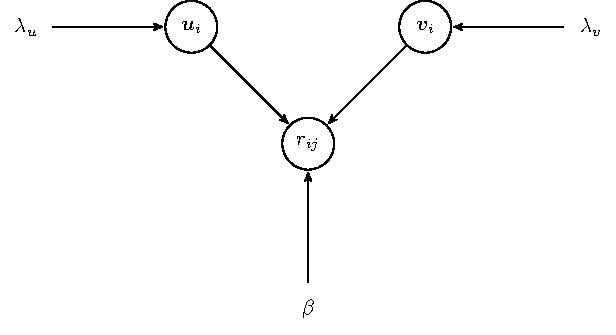
\includegraphics{includes/sampling-methods/matrix-factorization.pdf}
			\caption{Matrix Factorization as Latent Factor Model}
		\end{figure}

		The BMF model with Gaussian likelihood and Gaussian priors has local conjugacy. We can write the posteriors for the latent variables as follows

		\begin{align*}
			\prob{\vu_i \pipe \vR, \vV, \vU_{-i}}	&\qprop \prod_{j : r_{ij} \ne 0} \prob{r_{ij} \pipe \vu_i, \vv_j} \, \prob{\vu_i} \\
			\prob{\vu_j \pipe \vR, \vV, \vU_{-j}}	&\qprop \prod_{i : r_{ij} \ne 0} \prob{r_{ij} \pipe \vu_i, \vv_j} \, \prob{\vv_j}
		\end{align*} \br%

		This is very similar to bayesian linear regression and we can find compute the posterior which is of the form

		\begin{align*}
			\shortintertext{For user latent variables}
			\prob{\vu_i \pipe \vR, \vV}		&\eq \ND{\vu_i \pipe \vmu_{\vu_i}, \vSigma_{\vu_i}} \\
			\vSigma_{\vu_i}					&\eq \para{\lambda_u \vI_{K} + \beta \sum_{j : r_{ij} \ne 0} \vv_j \vv_j^T}^{-1} \\
			\vmu_{\vu_i}					&\eq \vSigma_{\vu_i} \para{\beta \sum_{j : r_{ij} \ne 0} r_{ij} \vv_j} \\
			\shortintertext{For item latent variables}
			\prob{\vv_j \pipe \vR, \vU}		&\eq \ND{\vv_j \pipe \vmu_{\vv_j}, \vSigma_{\vv_j}} \\
			\vSigma_{\vv_j}					&\eq \para{\lambda_v \vI_{K} + \beta \sum_{i : r_{ij} \ne 0} \vu_i \vu_i^T}^{-1} \\i
			\vmu_{\vu_i}					&\eq \vSigma_{\vv_j} \para{\beta \sum_{i : r_{ij} \ne 0} r_{ij} \vu_i}
		\end{align*} \br

		This idea is similar in spirit to alternating optimization methods (such as EM). 

	\end{ssubsection}

\end{ssection}

\begin{ssection}{Sampling from Distributions}

	We can approximate a distribution using a set of randomly drawn samples from it. However, it is not possible to directly sample \textit{difficult} distributions. Hence, we need sampling techniques that allow us to sample from such distributions \textit{e.g.} we sometimes might need to approximately infer / sample intractable posteriors. These samples can be used to approximate anything that depends on these distributions \textit{e.g.} expectations or posteriors.

	\begin{sssubsection}{Emperical Distribution}

		We sample using $L$ points $\set{\vz^{(l)}}_{l = 1}^{L}$ and the emperical distribution is defined as

		\begin{align*}
			\prob[L]{L}				&\eq \sum_{l = 1}^{L} w_l \func{\delta_{\vz^{(l)}}}{A} \\
			\shortintertext{where $\delta$ is the Dirac Delta function}
			\func{\delta_{\vz}}{A}	&\eq 
				\begin{cases}
					0	& \mt{if} \vz \in A \\
					1	& \mt{if} \vz \notin A
				\end{cases}
		\end{align*} \br%

		$w_l$ is the weight of a point. This distribution can be viewed as a histogram and the weight as the height of the histogram bar. This method can be used to sample from both simple as well as difficult distributions.

	\end{sssubsection}

	\begin{ssubsection}{Transformation Methods}

		Transformation methods are used to sample (mostly) generic or standard distributions, using simple distributions which can be easily sampled (such as uniform distribution). We essentially transform

		\begin{sssubsection}{Inverse CDF Method}

			This method uses the change of variable rule to transform a simple distribution to more complex distributions. Suppose we want to sample the random variable $z$ using a simpler distribution $x$, then we can write

			\begin{align*}
				\prob{z}	&\eq \prob{x} \abs{\derp{x}{z}} \\
				\shortintertext{if $x$ is a uniform distribution}
				x			&\eq \int_{-\infty}^{\hat{z}} \prob{z} dz = \func{F}{\hat{z}}
			\end{align*}

			Thus, we can first draw a random sample $x$ from $\func{Unif}{0, 1}$ and transform into $z$ using $\hat{z} = \funcinv{h}{u}$

		\end{sssubsection}

		\begin{sssubsection}{Box-Muller Method}

			This is a transformation technique to generate samples from two-dimensional Gaussian Distribution. The transformation is from the distribution $\func{Unif^2}{0, 1}$ to the desired one. \br%

			\begin{algo}{h!}{Box-Muller Transformation}

				\begin{enumerate}
					\item Assume two samples $u, v$ drawn from $U \sim \func{Unif}{0, 1}$ and $V \sim \func{Unif}{0, 1}$
					\item Transform these random variables into $R, \Theta$ such that $R = \sqrt{-2 \log{U}}$ and $\Theta = 2 \pi V$
					\item Since $\Theta$ is a linear transformation, we know $\Theta \sim \func{Unif}{0, 2 \pi}$
					\item For $R$
						\begin{align*}
							\prob{R \le r}			&\eq \prob{\sqrt{-2 \log{U}} \le r} \\
													&\eq 1 - \prob{U < \exp{- \frac{r^2}{2}}} \\
													&\eq 1 - \exp{- \frac{r^2}{2}} \\
							\\
							\implies \func[R]{f}{r}	&\eq r \exp{- \frac{r^2}{2}}
						\end{align*}
					\item Since $U$ and $V$ are independent, $R$ and $\Theta$ will also be independent. Hence $\func[R, \Theta]{f}{r, \theta} = \frac{1}{2 \pi} r \exp{- \frac{r^2}{2}}$
					\item We further transform these into two random variables $Z_1$ and $Z_2$
						\begin{align*}
							Z_1 = R \cos{2 \pi \Theta} && \mt{and} && Z_2 = R \sin{2 \pi \Theta}
						\end{align*}
					\item The join distribution of $Z_1, Z_2$ is given by
						\begin{align*}
							\func[Z_1, Z_2]{f}{z_1, z_2} \derp{z_1, z_2}{r, \theta}	&\eq \func[R, \Theta]{f}{r, \theta} \\
																					&\eq \brac{\frac{1}{\sqrt{2 \pi}} \exp{- \frac{z_1^2}{2}}} \brac{\frac{1}{\sqrt{2 \pi}} \exp{- \frac{z_2^2}{2}}} \\
																					&\eq \ND{z_1, z_2 \pipe \vzero, \vI_{2}}
						\end{align*}
				\end{enumerate}

			\end{algo}

			\clearpage

			It is also possible to transform Normal distrubition to any other gaussian distribution. Suppose a random variable $X \sim \ND{\vzero, \vI_{k}}$. Transform this into $Z \sim{\vmu, \vSigma}$ as follows

			\begin{align*}
				Z	\eq		\vmu + LX
			\end{align*}

			where $L$ is the Cholesky decomposition of $\vSigma$

			\note{Cholesky decomposition of $\vSigma$ will always exist as it is a positive definite matrix}

		\end{sssubsection}

	\end{ssubsection}

	\begin{ssubsection}{Rejection Sampling}

		Suppose we have a random variable with an intractable normalization factor, we can still sample it using rejection sampling. Consider a distribution $p(z)$ such that

		\begin{align*}
			\prob{z}	\eq \frac{\aprob{z}}{Z_p}
		\end{align*}

		where $Z_p$ is not computable. \br%

		In order to sample, we need a \textit{proposal distribution} $\func{q}{z}$ such that

		\begin{align*}
			M \func{q}{z} > \aprob{z}	&&	\forall\, z \quad \mt{where M is a constant}
		\end{align*}

		The steps to generate sample are as follows

		\begin{algo}{h!}{Rejection Sampling}

			\begin{enumerate}
				\item Sample a random variable $z_\ast$ from $\func{q}{z}$
				\item Sample a uniform random variable $u \sim \func{Unif}{0, M \func{q}{z_\ast}}$
				\item If $u \le \aprob{z_\ast}$, then \textit{accept} else \textit{reject}
			\end{enumerate}

		\end{algo}

		The proof of the algorithm can be seen as follows

		\begin{align*}
			\prob{\mt{accept} \pipe z}	&\eq	\frac{\aprob{z}}{M \func{q}{z}} \\
			\prob{z, \mt{accept}}		&\eq	\func{q}{z} \prob{\mt{accept} \pipe z} 	&\eq \frac{\aprob{z}}{M} \\
			\prob{\mt{accept}}			&\eq	\int \frac{\aprob{z}}{M} dz				&\eq	\frac{Z_p}{M} \\
			\prob{z \pipe \mt{accept}}	&\eq	\frac{\aprob{z}}{Z_p}					&\eq	\prob{z}
		\end{align*}

	\end{ssubsection}

\end{ssection}

\begin{ssection}{Expections via Monte Carlo Sampling}

	$\cZ$

\end{ssection}<++>

\end{document}
